\documentclass[UTF8,a4paper,12pt]{ctexart}
\usepackage{amsmath,amssymb,booktabs,graphicx,float,geometry}
\geometry{left=2.5cm,right=2.5cm,top=2.6cm,bottom=2.6cm}
\graphicspath{{../figures_enhanced/}}
\title{2020年全国大学生数学建模竞赛B题第一问增强图表稿}
\author{}
\date{}

\begin{document}
\maketitle

\section{第一问模型与求解结果}

第一问被建模为有限期资源约束状态模型，并等价展开为逐日整数网络流。模型以日期、位置、水和食物为状态，以现金为价值，统一表示行走、停留、挖矿和村庄补给。两关均由 HiGHS 求得零 MIP 间隙的全局最优解，并由独立规则引擎逐日复算。第一关最优终端财富为10470元，于第24天到达终点；第二关最优终端财富为12730元，于第30天到达终点。

\begin{figure}[H]
  \centering
  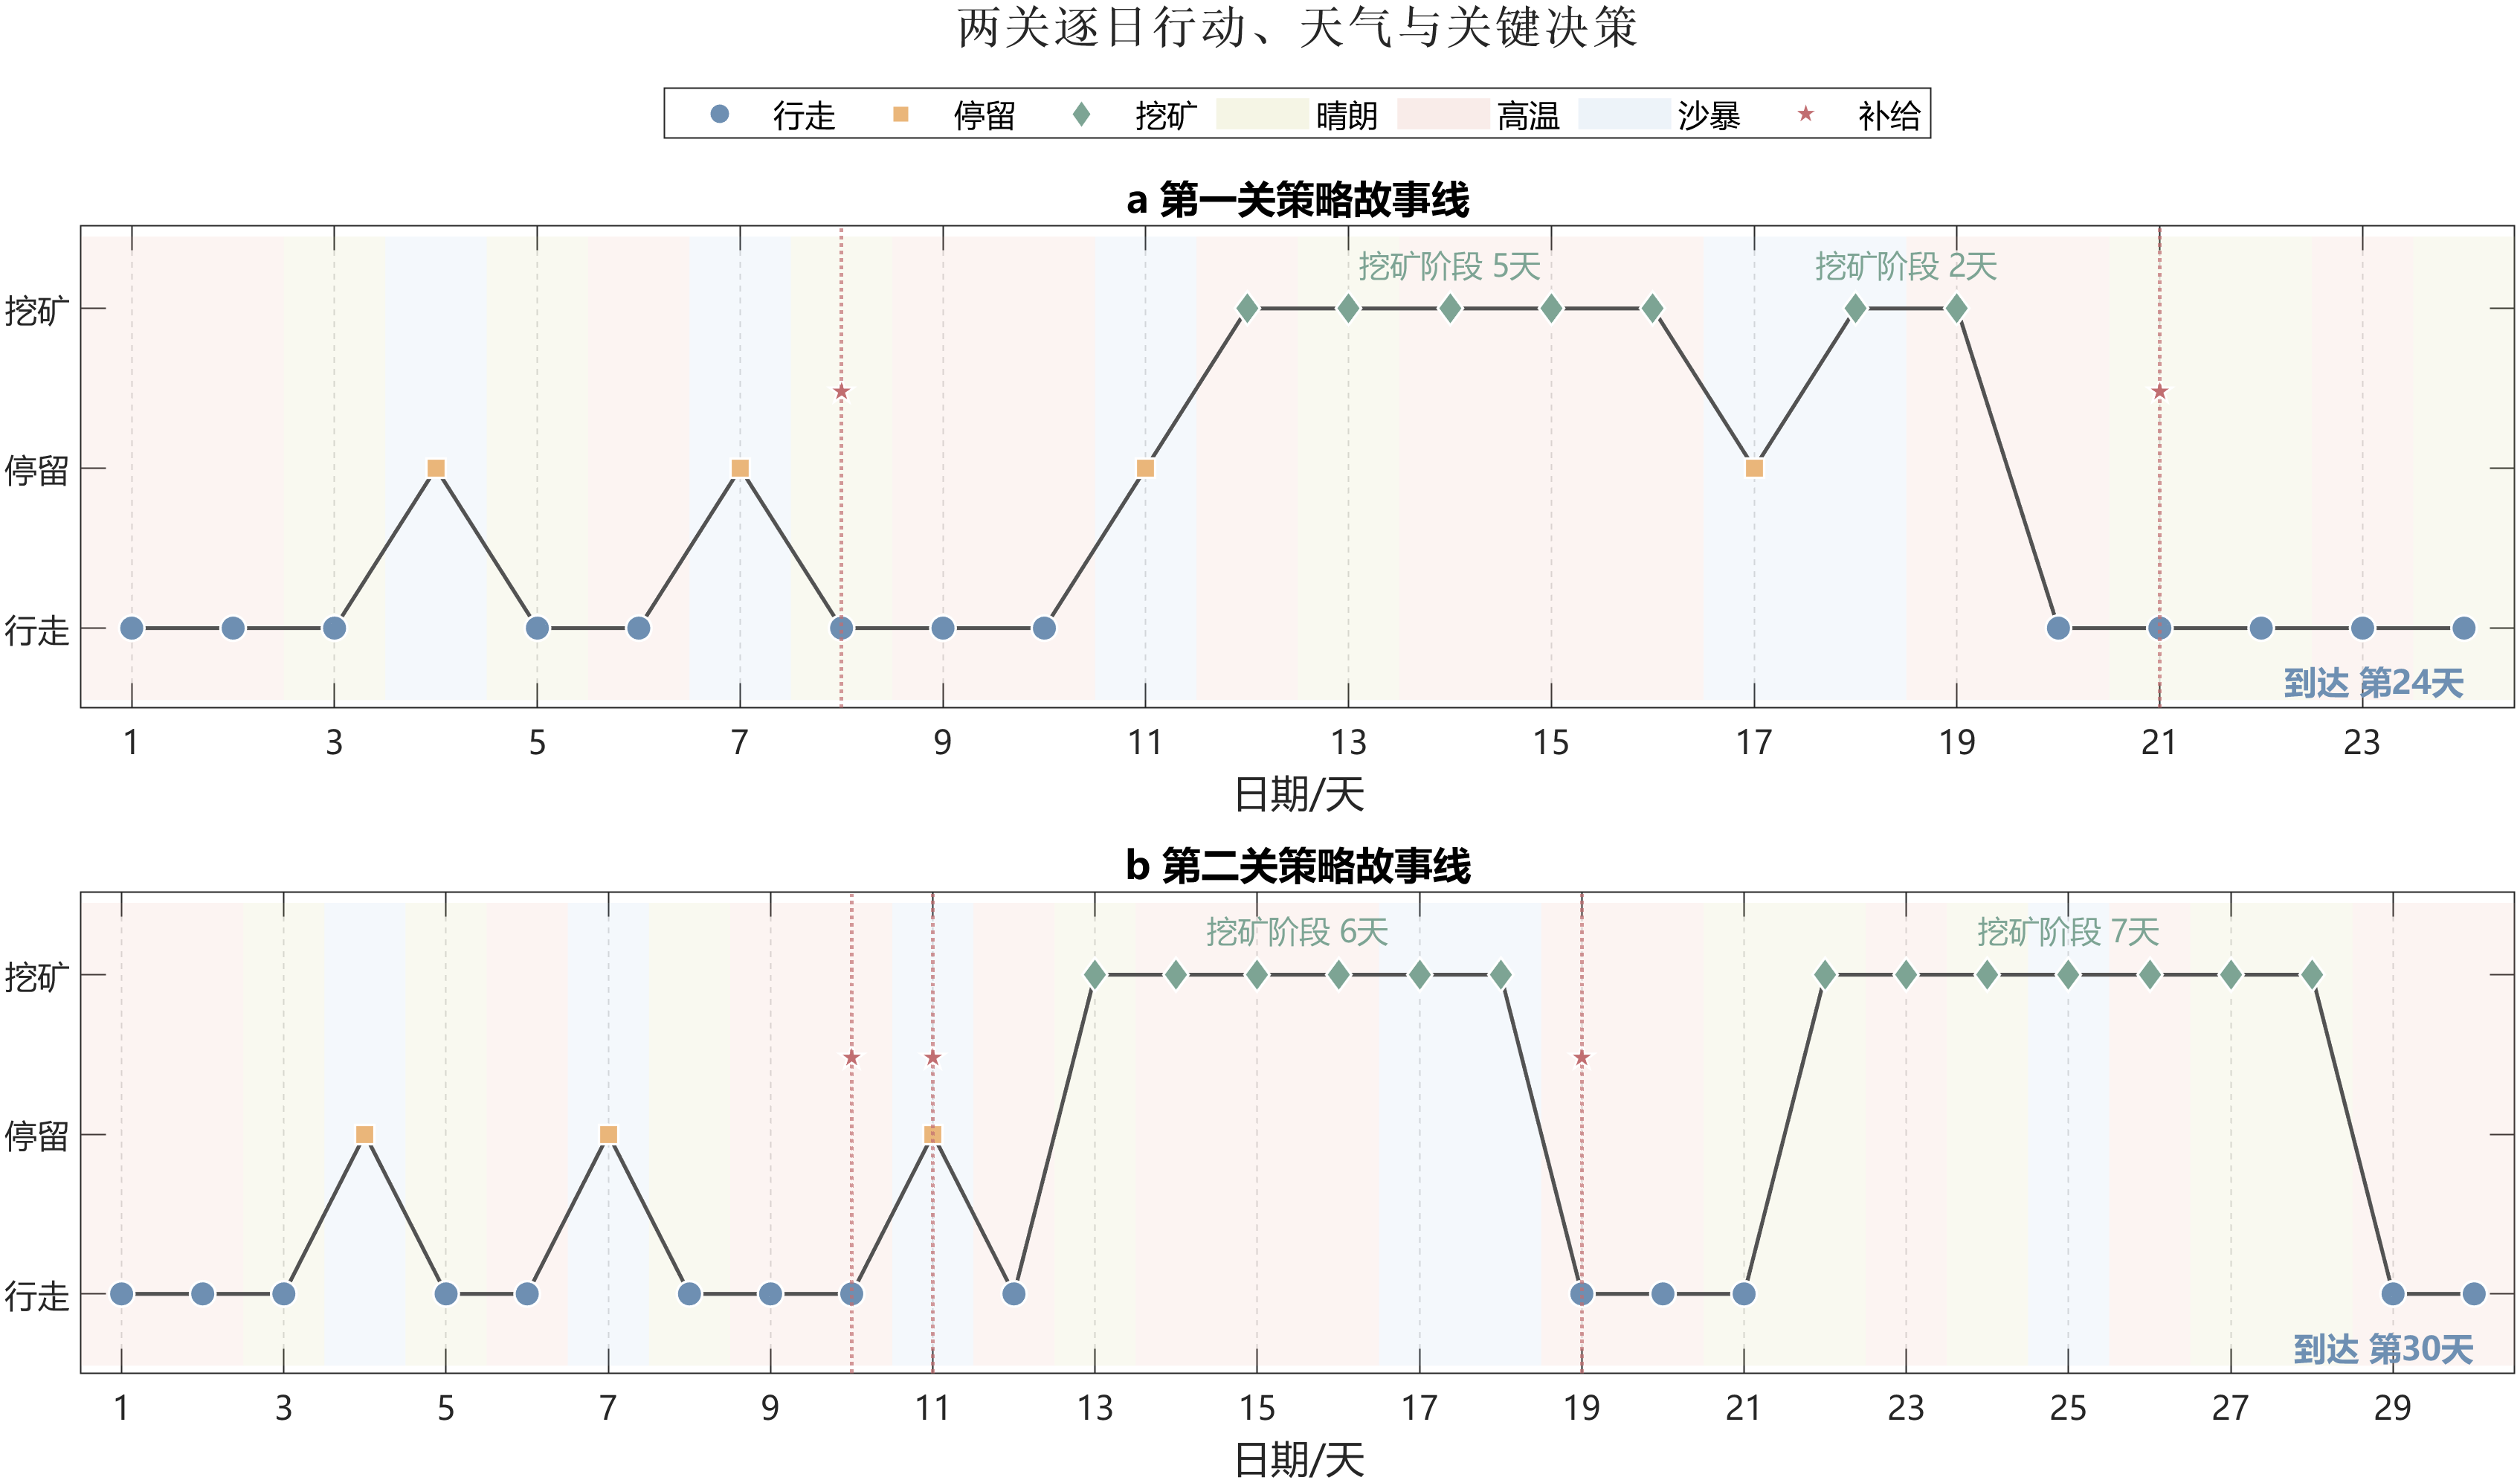
\includegraphics[width=0.98\textwidth]{fig_q1_strategy_storyboard.png}
  \caption{两关逐日行动、天气与关键决策}
\end{figure}

由图1可见，两关均在天气约束下完成行走、停留和挖矿状态的逐日切换。第一关形成5天和2天两段挖矿阶段，第二关形成6天和7天两段挖矿阶段；补给节点与后续挖矿或末段行走紧密衔接。

\begin{figure}[H]
  \centering
  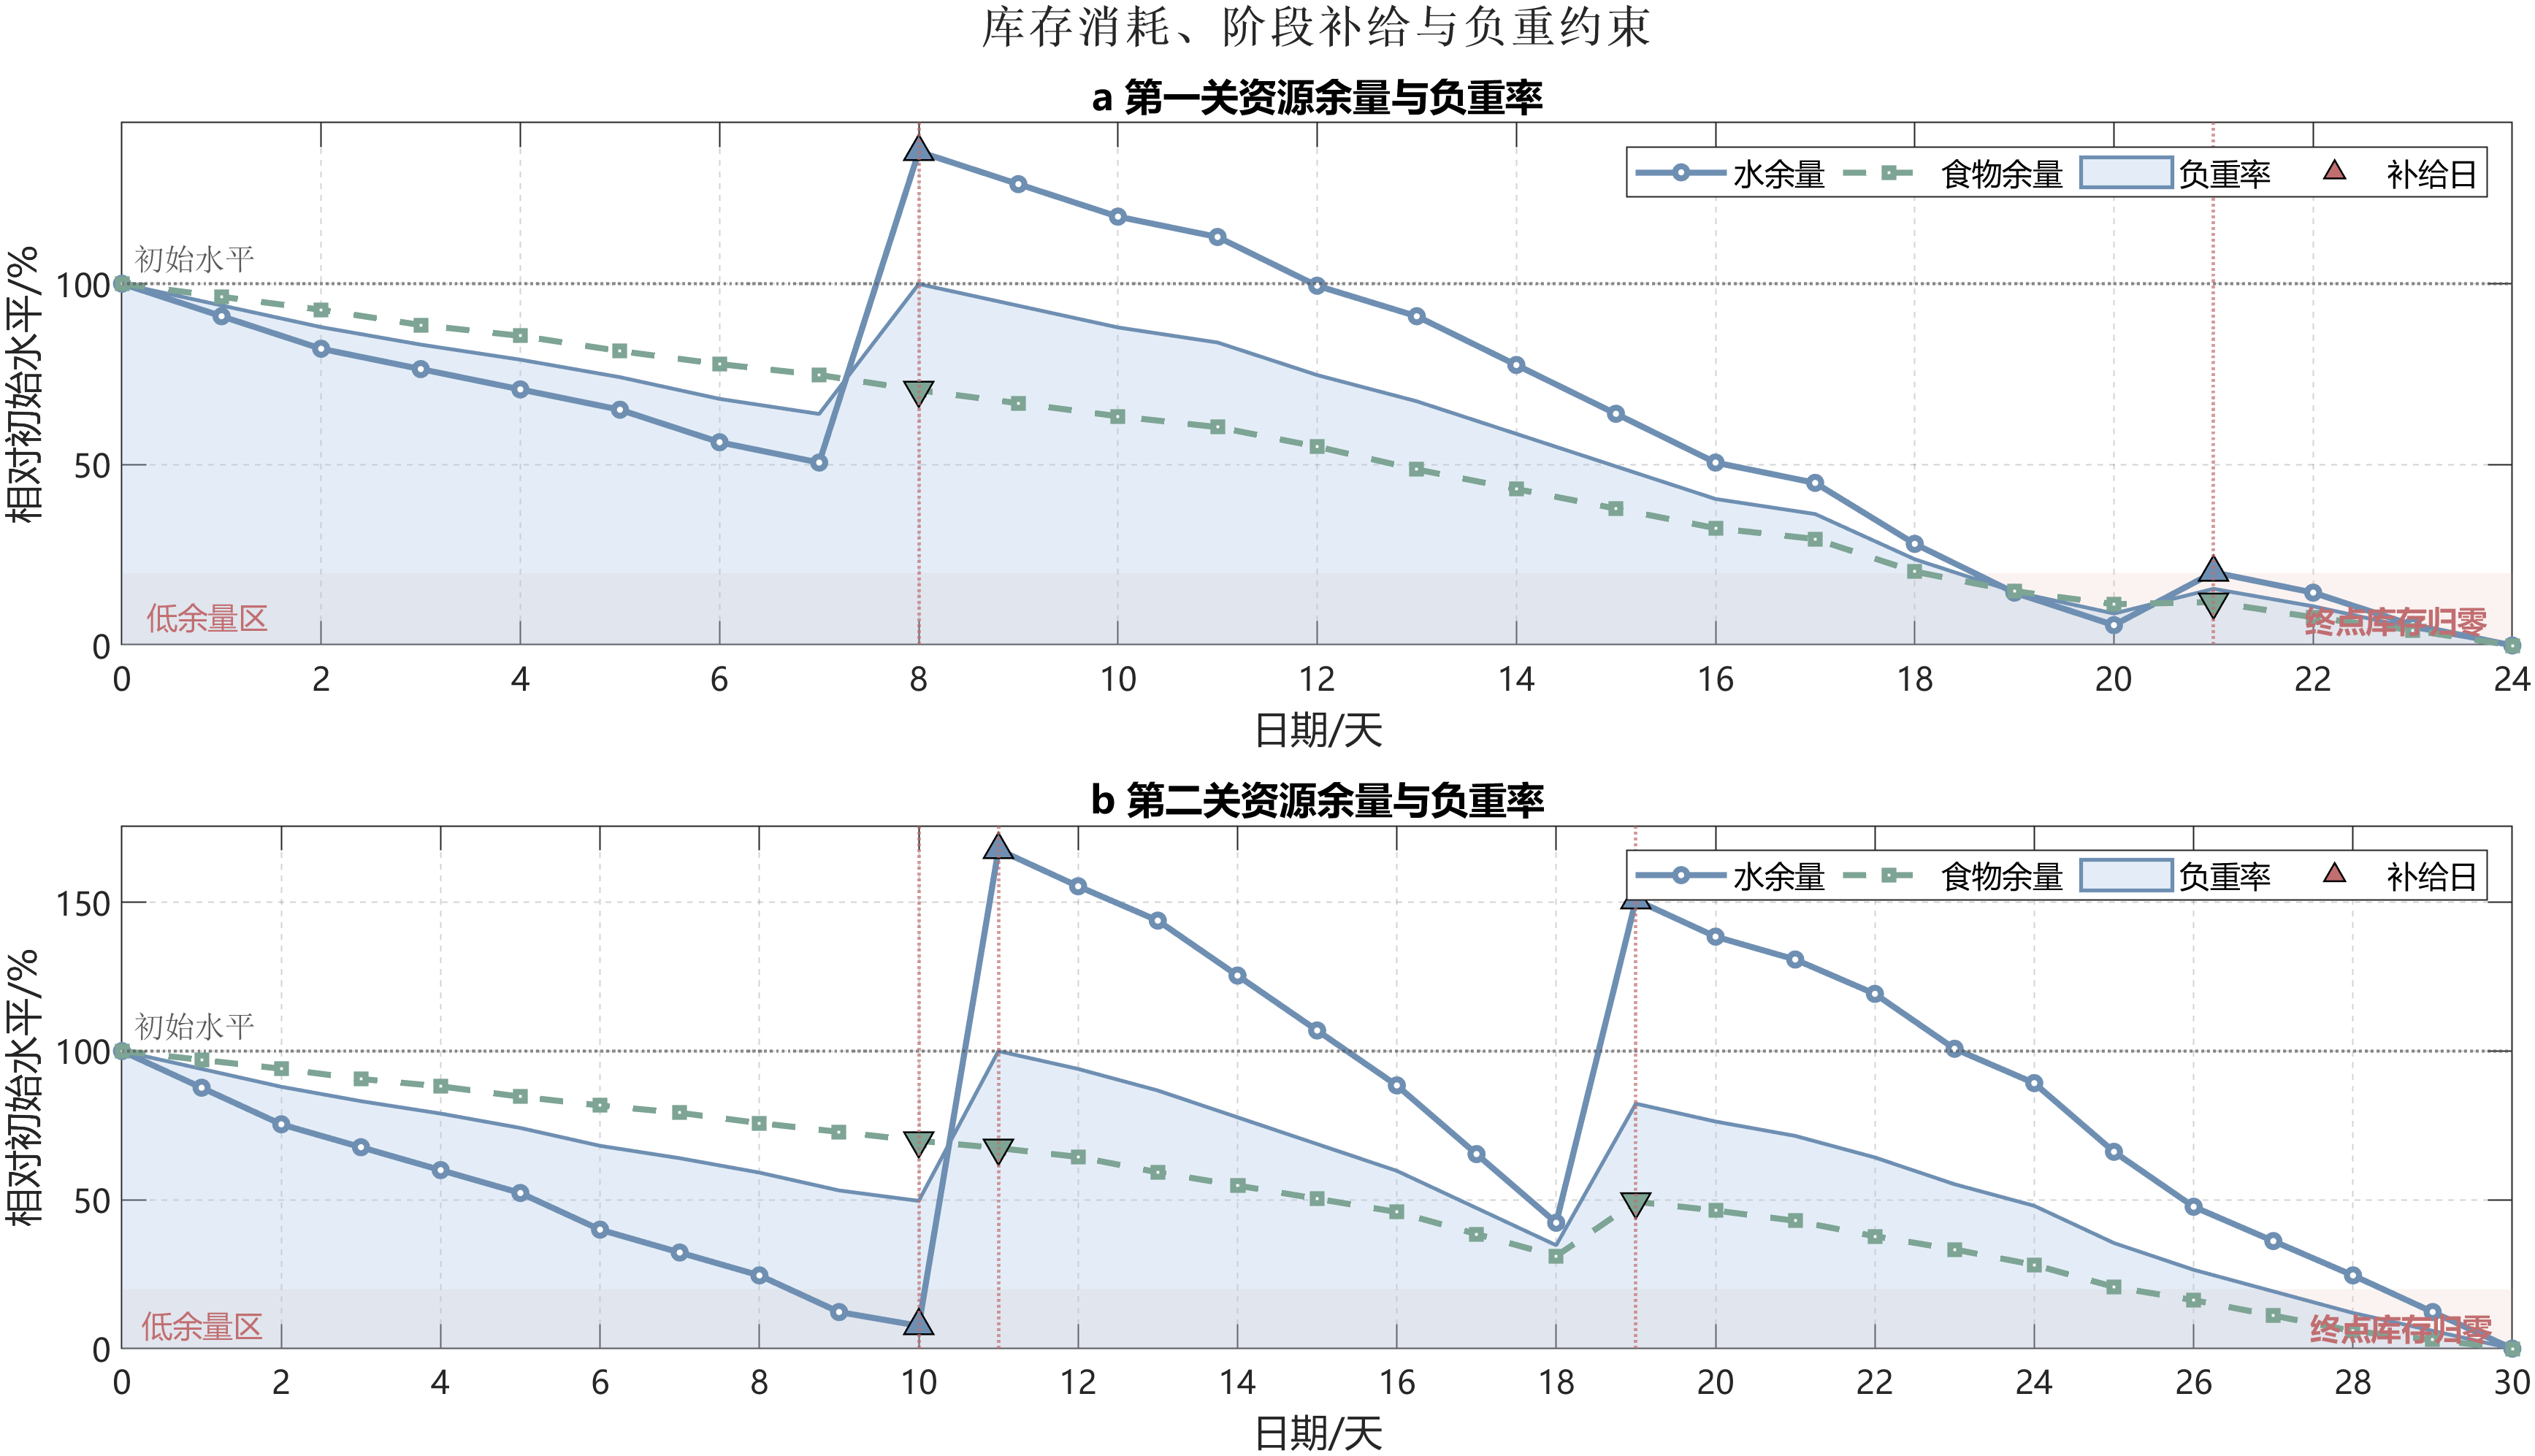
\includegraphics[width=0.98\textwidth]{fig_q1_resource_ribbon.png}
  \caption{库存消耗、阶段补给与负重约束}
\end{figure}

图2将水、食物和负重统一表示为相对初始水平。两关第0天负重率均为100\%，补给日库存明显跃升，随后随行走和挖矿持续下降，最终水和食物均精确归零。

\begin{figure}[H]
  \centering
  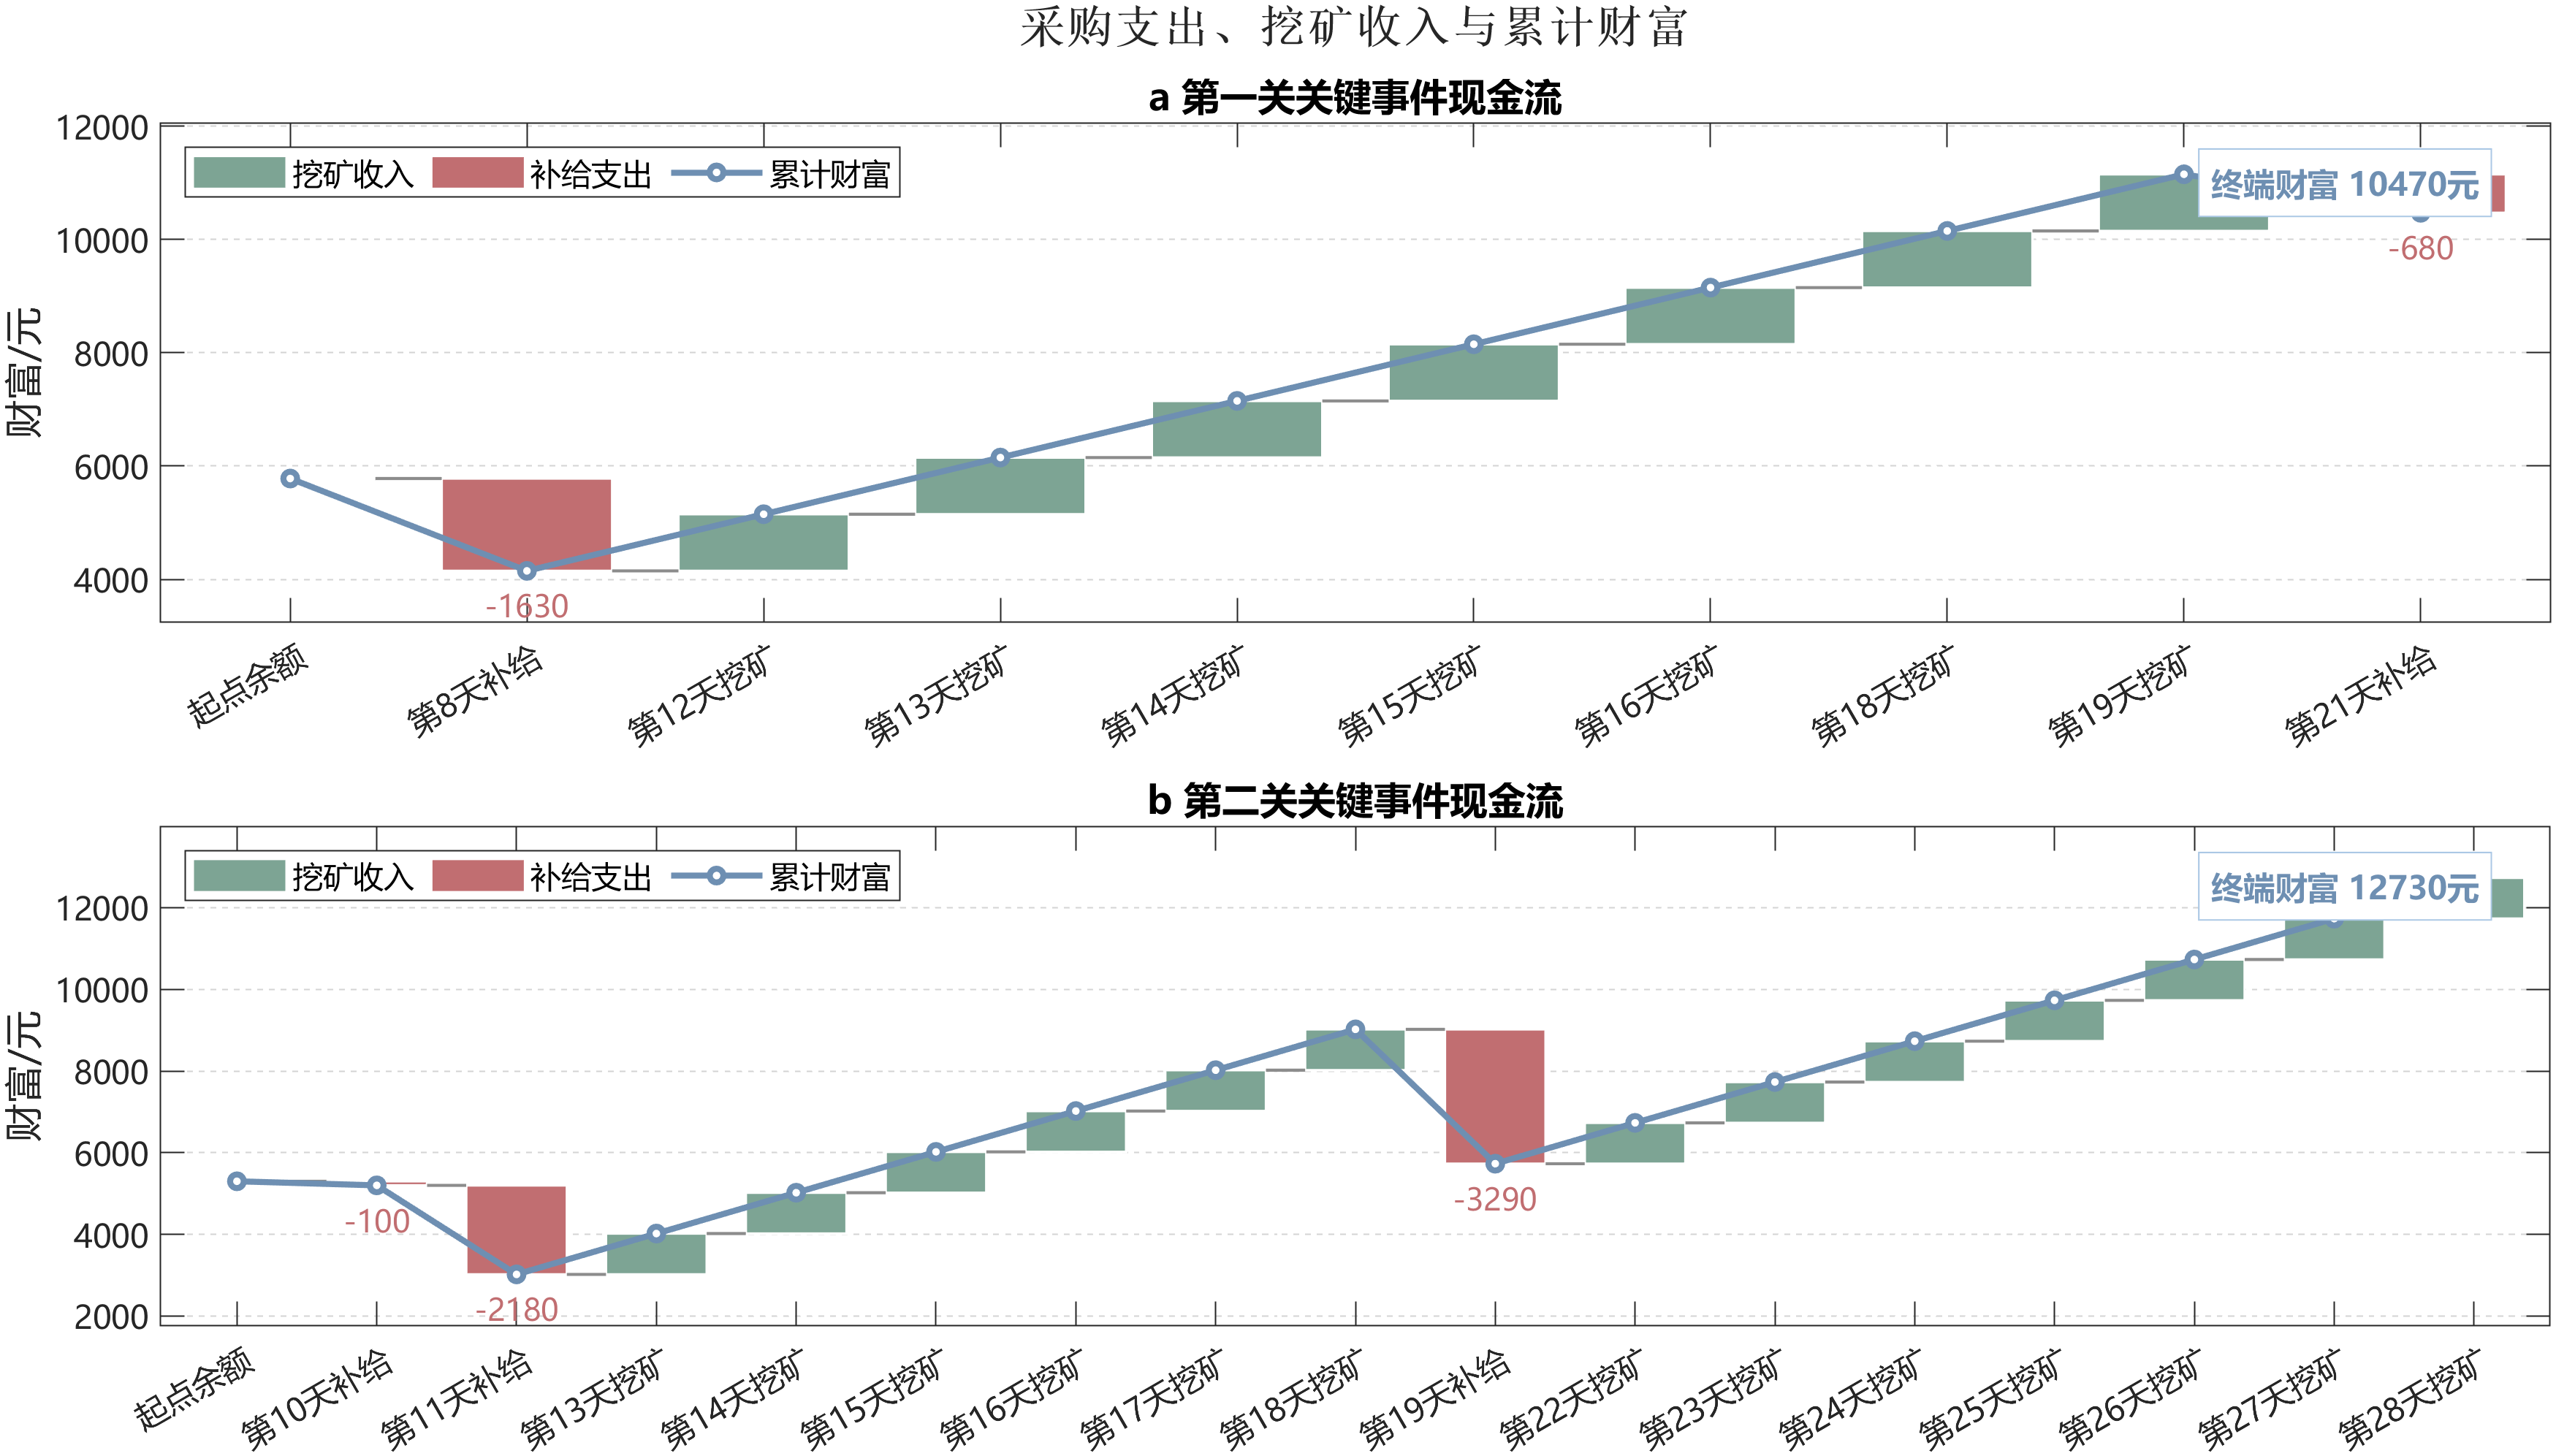
\includegraphics[width=0.98\textwidth]{fig_q1_cashflow_waterfall.png}
  \caption{采购支出、挖矿收入与累计财富}
\end{figure}

图3只保留资金变化事件。第一关两次途中补给分别支出1630元和680元，7个挖矿日带来7000元收入；第二关三次途中补给共支出5570元，13个挖矿日带来13000元收入，因此终端财富达到12730元。

\begin{figure}[H]
  \centering
  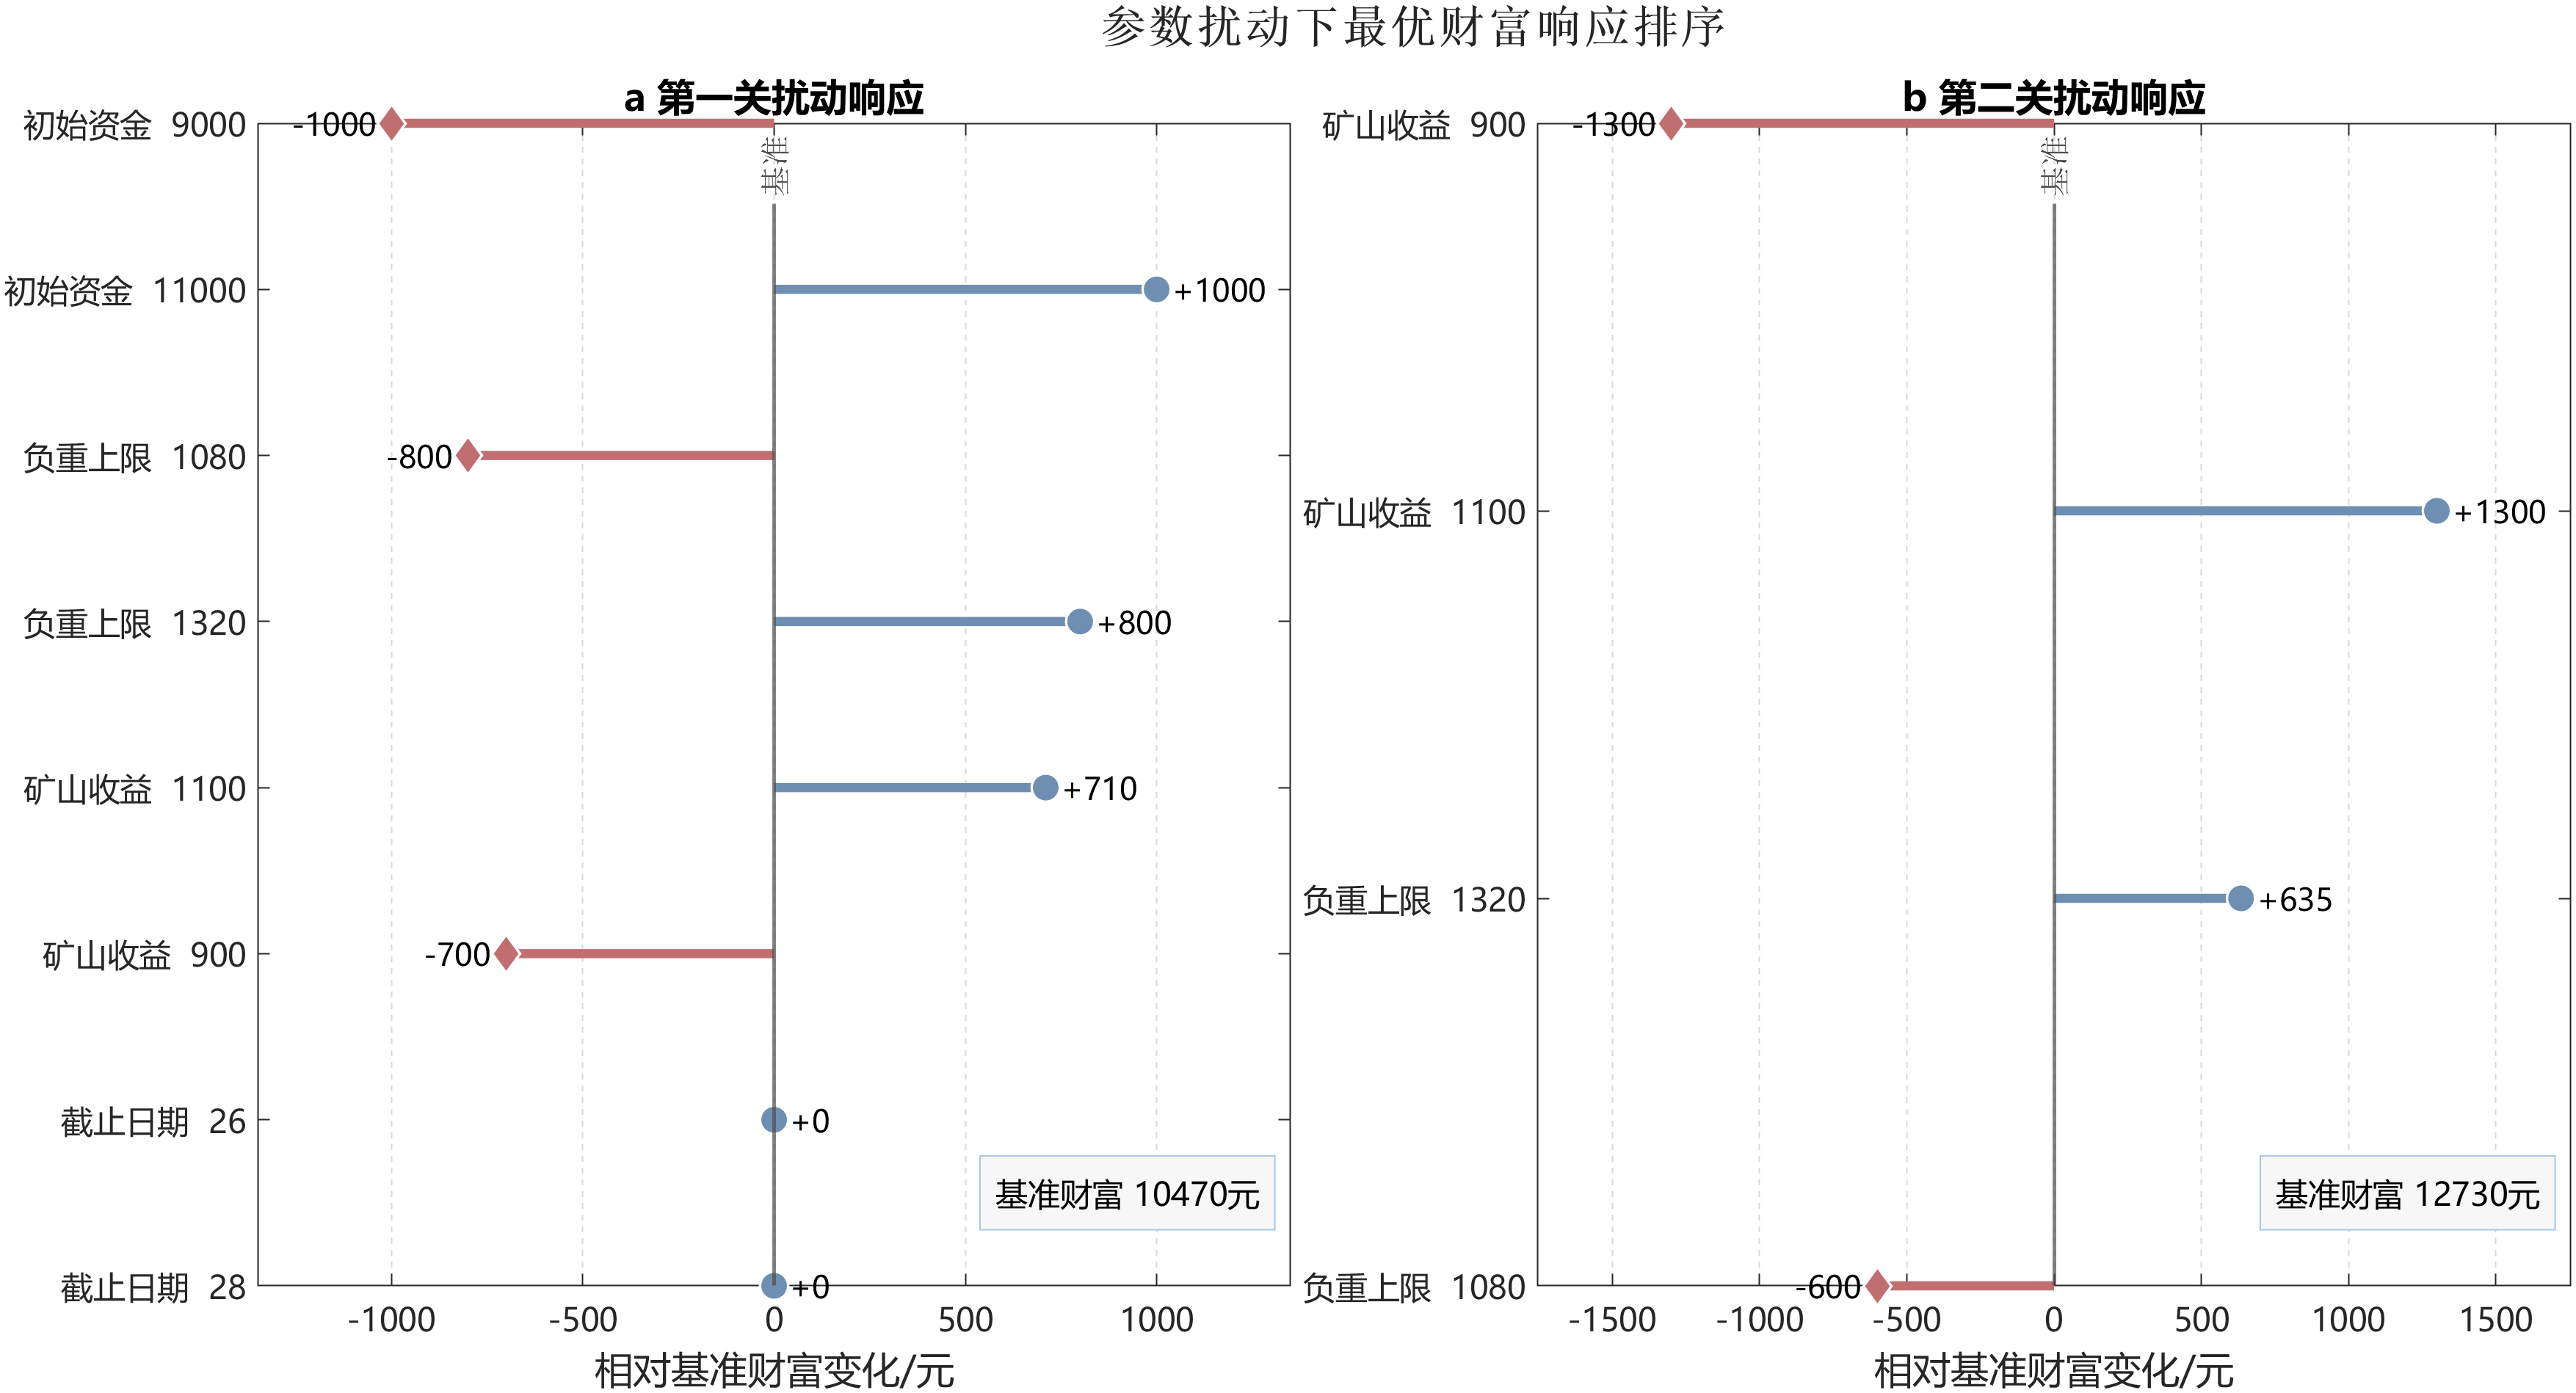
\includegraphics[width=0.98\textwidth]{fig_q1_sensitivity_lollipop.png}
  \caption{参数扰动下最优财富响应排序}
\end{figure}

图4显示，第一关财富对初始资金和负重上限的扰动变化较大，而截止日期在已计算区间内不改变最优财富。第二关对矿山收益最敏感，矿山收益每变化100元，最优财富变化1300元。

\begin{figure}[H]
  \centering
  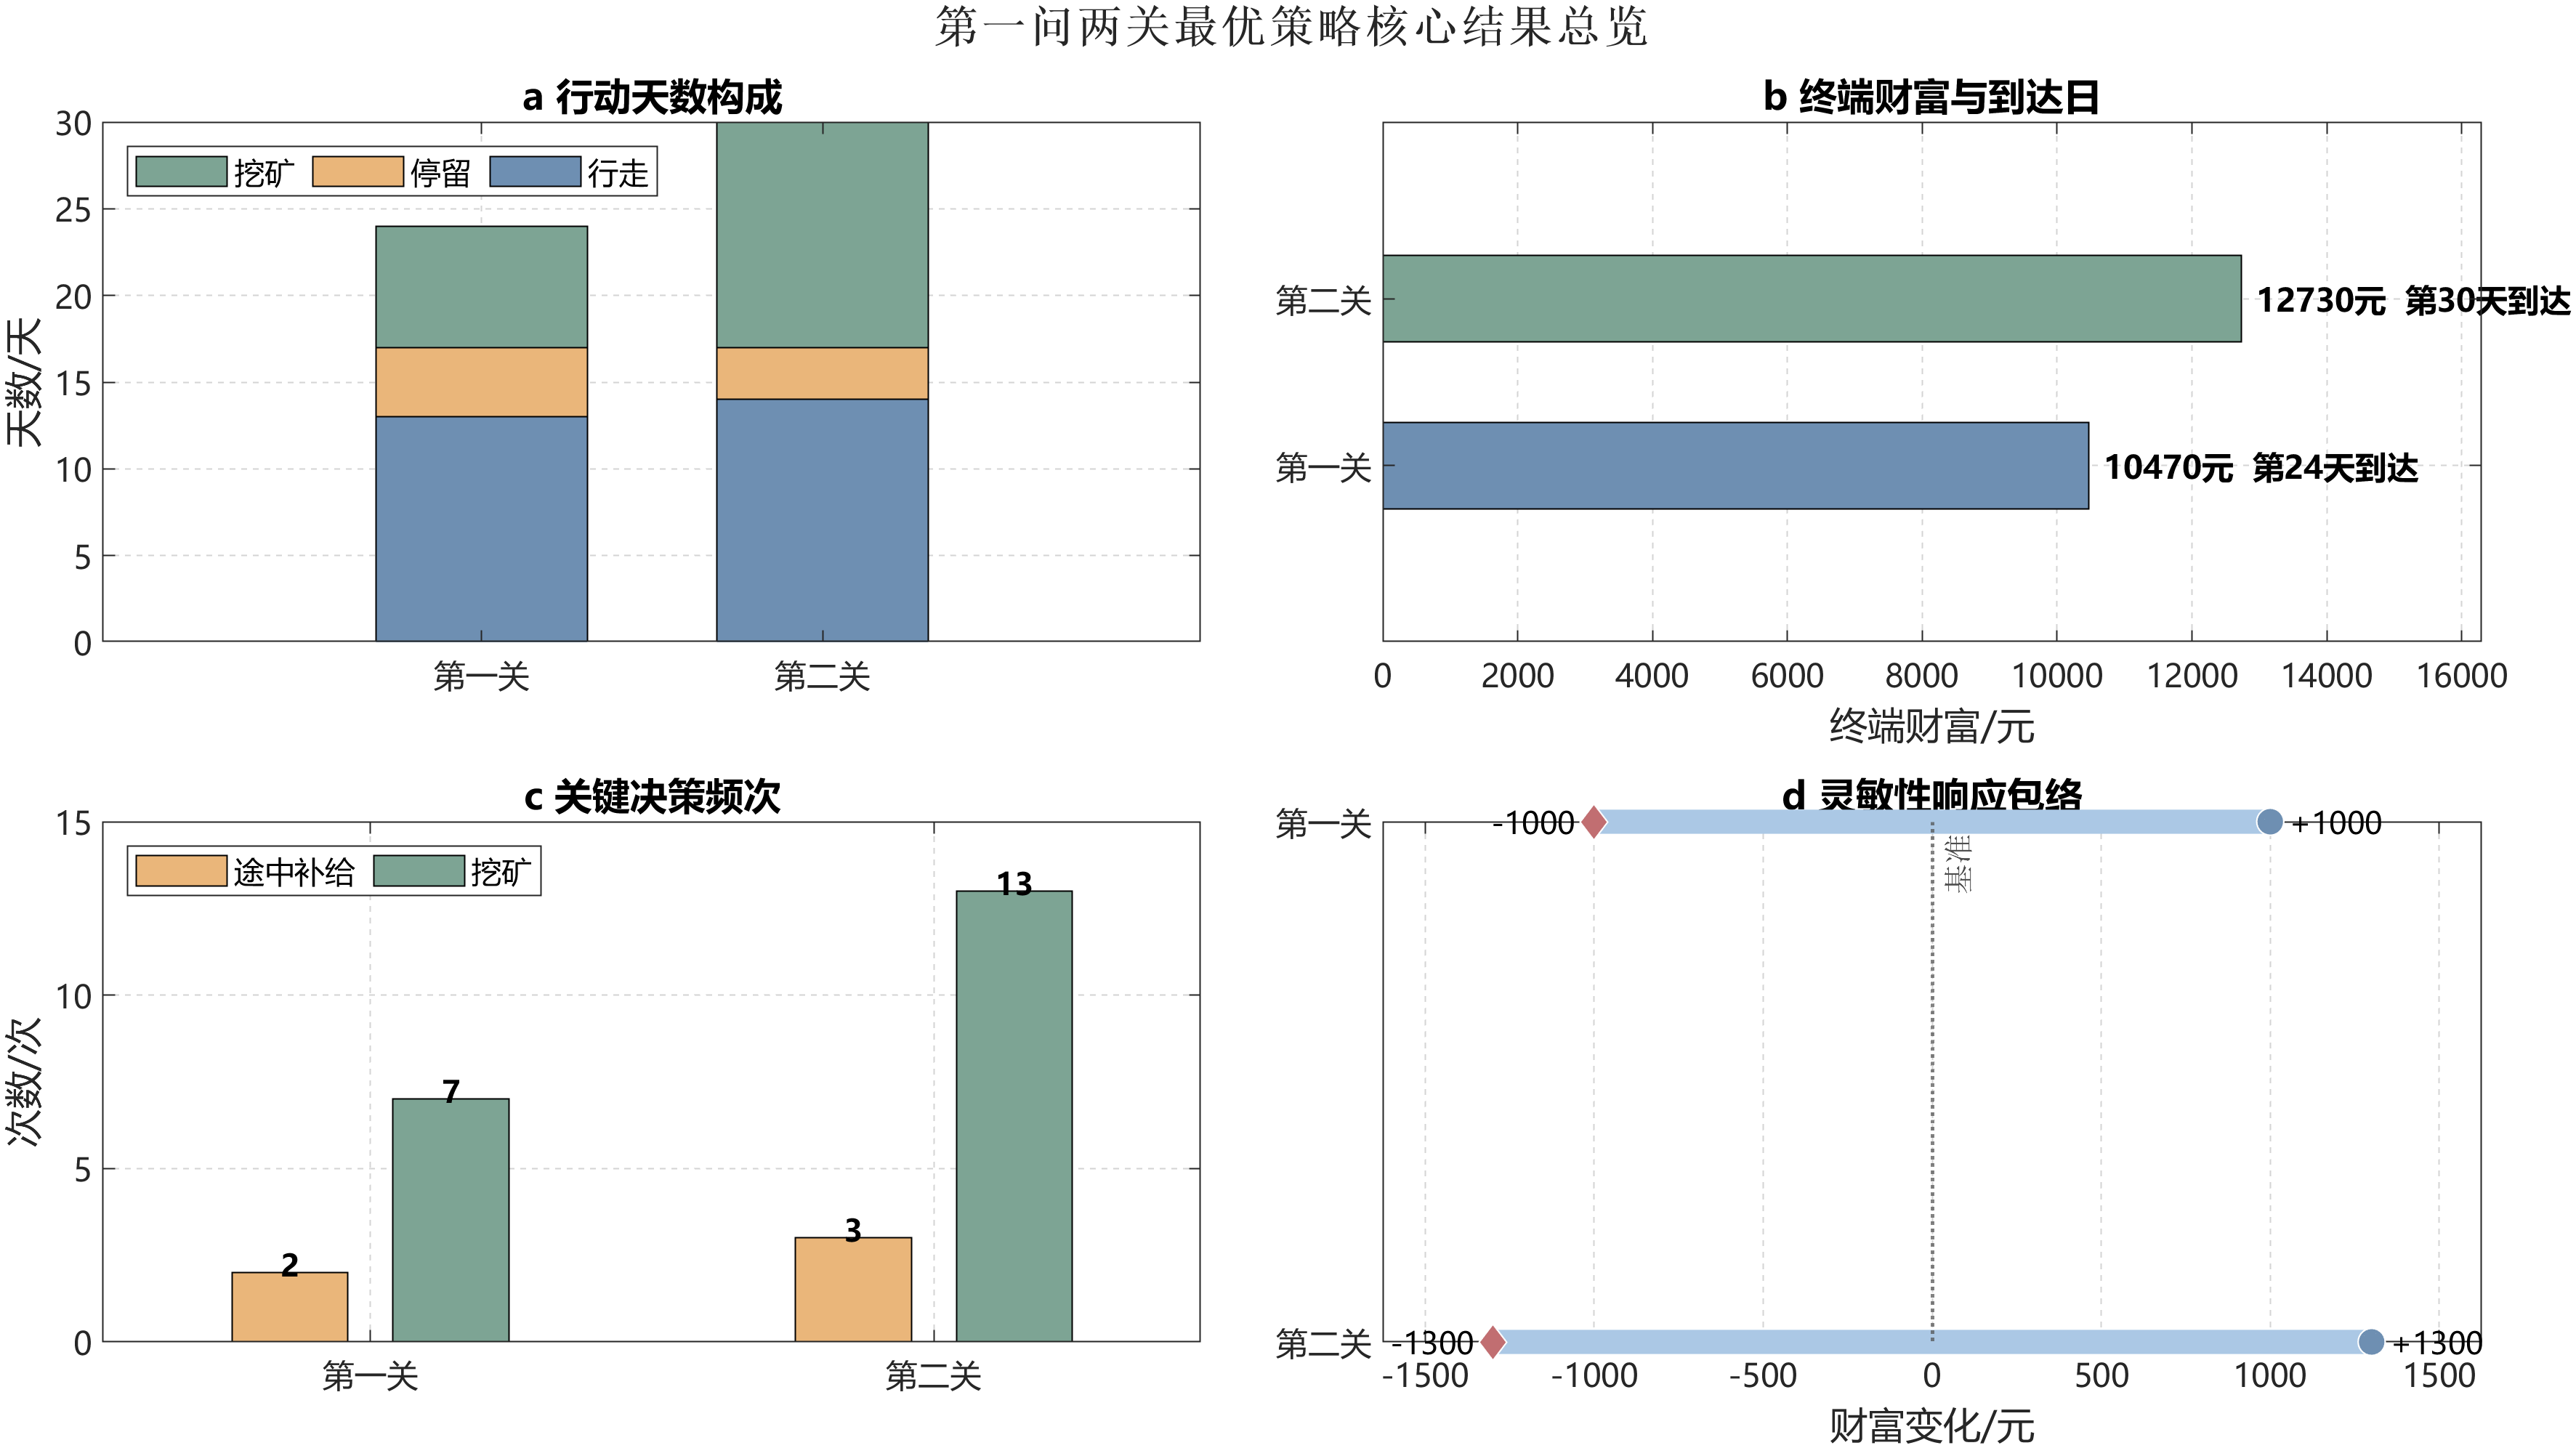
\includegraphics[width=0.98\textwidth]{fig_q1_strategy_dashboard.png}
  \caption{第一问两关最优策略核心结果总览}
\end{figure}

总览图表明，第二关比第一关多6天、增加6个挖矿日和1次途中补给，最终财富高2260元；与此同时，其参数扰动响应范围也更宽，说明更高收益伴随更强的参数敏感性。

\section{可靠性与适用边界}

两关逐日策略均满足邻接、沙暴禁行、资源非负、负重不超限、现金非负、村庄采购和终点吸收约束。灵敏性图只使用完整整数模型实际重求解的参数点，不对未计算区间进行插值。模型依赖全时段天气完全已知，不能直接替代未知天气下的在线决策模型。

\end{document}
